\documentclass[solutionorbox, answers]{exam}
% \documentclass[solutionorbox]{exam}

%%%%%%%%%%%%%%%%%%%%%%%%%%%%%%%%%%%%%%%%%%%%%%%%%%%%%%%%%%%%%%%
% Update to change header
\newcommand{\courseName}{CS 577}
\newcommand{\assignmentName}{Assignment 1 -- Discrete Review}
\newcommand{\semester}{Summer 2025}
%%%%%%%%%%%%%%%%%%%%%%%%%%%%%%%%%%%%%%%%%%%%%%%%%%%%%%%%%%%%%%%

\usepackage[utf8]{inputenc}
\usepackage[T1]{fontenc}

\usepackage{amsmath}
\usepackage{amsfonts}
\usepackage{amsthm}
\usepackage{booktabs}
\usepackage{tkz-graph}
\usepackage[ruled]{algorithm2e}
\usepackage{graphicx}
\usepackage{multicol}

\usepackage{listings}
\lstset{basicstyle=\ttfamily,
  showstringspaces=false,
  commentstyle=\color{red},
  keywordstyle=\color{blue}
}

\usepackage{hyperref}

\pagestyle{headandfoot}
\runningheadrule
\firstpageheader{\courseName}{\huge \assignmentName}{\semester}
\runningheader{\courseName}
{\assignmentName}
{\semester}
\firstpagefooter{}{}{}
\runningfooter{}{Page \thepage\ of \numpages}{}

\begin{document}

\begin{center}
\fbox{\parbox{5.5in}{\centering
Answer the questions in the boxes provided on the
question sheets. If you run out of room for an answer,
add a page to the end of the document. \\
\vspace{0.1in}
Related Readings:
\begin{itemize}
\item Proof Primer: \url{https://canvas.wisc.edu/courses/434199/files/43389378}
\item  CS240 Readings: \url{http://pages.cs.wisc.edu/~hasti/cs240/readings/}
\end{itemize}

}}
\end{center}
\vspace{0.1in}
\makebox[0.48\textwidth]{Name:\enspace\hrulefill} \qquad
\makebox[0.48\textwidth]{Wisc id:\enspace\hrulefill}

\begin{questions}

\section*{Induction}
\label{sec:induction}

\question
Prove the following by induction.

\begin{parts}
  \part
  $\sum_{i = 1}^n i = n(n+1)/2$
  \begin{solutionbox}{\stretch{1}}\\
  \end{solutionbox}
  
  \part
  $\sum_{i = 1}^n i^2 = n(n+1)(2n+1)/6$
  \begin{solutionbox}{\stretch{1}}\\
    \end{solutionbox}
    
\newpage
  \part
  $\sum_{i = 1}^n i^3 = n^2(n+1)^2/4$
    \begin{solutionbox}{\stretch{1}}\\
  \end{solutionbox}
\end{parts}

\section*{Graphs and Trees}
\label{sec:graphs-trees}

\question 
Give the adjacency matrix, adjacency list, edge list, and incidence matrix for the following graph. \\
\begin{minipage}{0.3\linewidth}
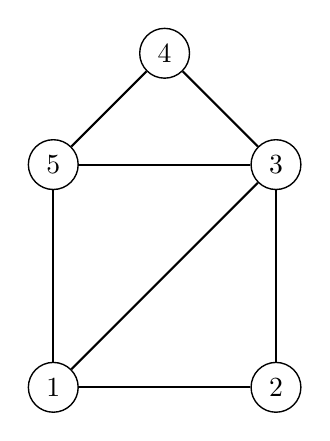
\begin{tikzpicture}
\GraphInit[vstyle=Normal]
\SetGraphUnit{2}
\begin{scope}[rotate=-135]
\Vertices{circle}{1,2,3,5}
\end{scope}
\NOEA[unit=1.414](5){4}
\Edges(1,2,3,5,4,3,1,5)
\end{tikzpicture}
\end{minipage}
\qquad
\begin{minipage}{0.6\linewidth}
\begin{solutionbox}{3.8in}                                                                          \\
\end{solutionbox}
\end{minipage}
\question
How many edges are there is a complete graph of size $n$? Prove by induction.

\begin{solutionbox}{3.8in}
\end{solutionbox}

\question
Draw all possible (unlabelled) trees with 4 nodes.

\begin{solutionbox}{3.8in}
\end{solutionbox}

\question
Show by induction that, for all trees, $|E| = |V| - 1$.

\begin{solutionbox}{3.8in}
\end{solutionbox}

\section*{Proofs}
\label{sec:proofs}

\question
Show that $2x$ is even for all $x \in \mathbb{N}$.

\begin{parts}
  \part
  By direct proof.
  \begin{solutionbox}{2in}
  \end{solutionbox}
  
  \part
  By contradiction.
    \begin{solutionbox}{2in}
    \end{solutionbox}
  \end{parts}

\question
For all $x,y \in \mathbb{R}$, show that $|x + y| \le |x| + |y|$. (Hint: use proof by cases.)
\begin{solutionbox}{3in}
\end{solutionbox}

\section*{Program Correctness (and Invariants)}
\label{sec:program-correctness}

\question
For the following algorithms, describe the loop invariant(s) and prove that they are sound and complete.
\begin{parts}
  \part 
  \begin{algorithm}[H]
    \DontPrintSemicolon
    \KwIn{$a$: A non-empty array of integers (indexed starting at 1)}
    \KwOut{The smallest element in the array}
    \Begin{
      $min \gets \infty$\;
      \For{$i \gets 1$ \KwTo len($a$)}{
        \If{$a[i] < min$} {
          $min \gets a[i]$\; 
        }
      }
      \Return{$min$}\;
    }
    \caption{findMin}
  \end{algorithm}
  \begin{solutionbox}{5.9in} 
  \end{solutionbox}

    \part 
  \begin{algorithm}[H]
    \DontPrintSemicolon
    \KwIn{$a$: A non-empty array of integers (indexed starting at 1)}
    \KwOut{$a$ sorted from largest to smallest}
    \SetKw{Break}{break}
    \Begin{
      \For{$i \gets 2$ \KwTo len($a$)}{
        $val \gets a[i]$\;
        \For{$j \gets 1$ \KwTo $i - 1$}{
          \If{$val > a[j]$} {
            shift $a[j..i-1]$ to $a[j+1..i]$\;
            $a[j] \gets val$\;
            \Break
          }
        }
      }
      \Return{$a$}\;
    }
    \caption{InsertionSort}
  \end{algorithm}
  \begin{solutionbox}{5.9in}
  \end{solutionbox}
  
\end{parts}

\section*{Coding Question: Hello World}

Most assignments will have a coding question. You can code in C, C++, C\#, Java, Python, or Rust. You will submit a Makefile and a source code file.
\vspace{-0.5cm}

\paragraph{Makefile:} In the Makefile, there needs to be a build command and a run command. Below is a sample Makefile for a C++ program. You will find this Makefile in assignment details. Download the sample Makefile and edit it for your chosen programming language and code.

\lstinputlisting[language=Make]{Makefile}

\newpage
\question{\bf{HelloWorld Program Details}}
%\paragraph

The input will start with a positive integer, giving the number of instances that follow. For each instance, there will be a string. For each string $s$, the program should output Hello, $s$! on its own line.

A sample input is the following:
\begin{verbatim}
3
World
Marc
Owen
\end{verbatim}

The output for the sample input should be the following:
\begin{verbatim}
Hello, World!
Hello, Marc!
Hello, Owen!
\end{verbatim}

\newpage


\section*{Asymptotic Analysis}

  \question \textit{Kleinberg, Jon. Algorithm Design (p. 67, q. 3, 4).} Take the following list of functions and arrange them in ascending order of growth rate. That is, if function $g(n)$ immediately follows function $f(n)$ in your list, then it should be the case that $f(n)$ is $O(g(n))$. 

\begin{parts}
  \part
  $f_1(n) = n^{2.5}$ \\
  $f_2(n) = \sqrt{2n}$ \\
  $f_3(n) = n + 10$ \\
  $f_4(n) = 10n$ \\
  $f_5(n) = 100n$ \\
  $f_6(n) = n^2 \log{n}$
  \begin{solutionbox}{1in} \vspace{1em} \\
  \end{solutionbox}
  
  \part
  $g_1(n) = 2^{\log{n}}$ \\
  $g_2(n) = 2^n$ \\
  $g_3(n) = n(\log{n})$ \\
  $g_4(n) = n^{4/3}$ \\
  $g_5(n) = n^{\log{n}}$ \\
  $g_6(n) = 2^{(2^n)}$ \\
  $g_7(n) = 2^{(n^2)}$
  \nopagebreak
  \begin{solutionbox}{1in} \vspace{1em} \\
  \end{solutionbox}
  
\end{parts}

\pagebreak

  \question \textit{Kleinberg, Jon. Algorithm Design (p. 68, q. 5).} Assume you have a non-decreasing function $f$ such that $f(n) \ge 1$ and a non-decreasing function $g$ such that $g(n) \geq 2$. Also, assume that $f(n)$ is $O(g(n))$. For each of the following statements, decide whether you think it is true or false and give a proof or counterexample.

\begin{parts}
\part
    $f(n)^2$ is $O(g(n)^2)$
    
    \nopagebreak
    \begin{solutionbox}{1.8in} \vspace{1em} \\
  \end{solutionbox}


    \part 
    $2^{f(n)}$ is $O(2^{g(n)})$
    
    \nopagebreak
    \begin{solutionbox}{1.8in} \vspace{1em}                                                           \\
    \end{solutionbox}
  \part
  $\log_2{f(n)}$ is $O(\log_2{g(n)})$ 

  \begin{solutionbox}{3in} \vspace{1em} \\
  \end{solutionbox}
  
  
\end{parts}

\pagebreak

\question \textit{Kleinberg, Jon. Algorithm Design (p. 68, q. 6).} You're given an array $A$ consisting of $n$ integers. You'd like to output a two-dimensional $n$-by-$n$ array $B$ in which $B[i, j]$ (for $i < j$) contains the sum of array entries $A[i]$ through $A[j]$ — that is, the sum $A[i]+ A[i + 1]+... + A[j]$. (Whenever $i \geq j$, it doesn't matter what is output for $B[i,j]$.)  
Here's a simple algorithm to solve this problem. 

\begin{lstlisting}
for i = 1 to n
  for j = i + 1 to n  
    add up array entries A[i] through A[j]
    store the result in B[i, j]
  endfor  
endfor 
\end{lstlisting}

\begin{parts}

\part For some function $f$ that you should choose, give a bound of the form $O(f(n))$ on the running time of this algorithm on an input of size $n$ (i.e., a bound on the number of operations performed
by the algorithm).

\begin{solutionbox}{\stretch{1}}
\end{solutionbox}

\part For this same function $f$, show that the running time of the algorithm on an input of size $n$ is also $\Omega(f(n))$. (This shows an asymptotically tight bound of $\Theta(f(n))$ on the running time.)

\begin{solutionbox}{\stretch{7}}    
\end{solutionbox}

\pagebreak

\part Although the algorithm provided is the most natural way to solve the problem, it contains some highly unnecessary sources of inefficiency. Give a different algorithm to solve this problem, with an asymptotically better running time. In other words, you should design an algorithm with running time $O(g(n))$, where $\lim_{n \to \infty}{\frac{g(n)}{f(n)}} = 0$. 

\begin{solutionbox}{\stretch{1}}    \vspace{1em}     \\
\end{solutionbox}

\end{parts}


\pagebreak
\section*{Graphs}

\question Given the following graph, list a possible order of traversal of nodes by breadth-first search and by depth-first search. Consider node 1 to be the starting node.

\begin{minipage}{0.3\linewidth}
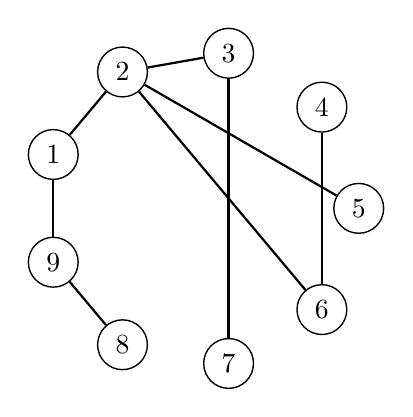
\begin{tikzpicture}
\GraphInit[vstyle=Normal]
\SetGraphUnit{2}
\Vertices{circle}{5,4,3,2,1,9,8,7,6}
\Edges(8,9,1,2,5)
\Edges(2,3,7)
\Edges(4,6)
\Edges(2,6)
\end{tikzpicture}
\end{minipage}
\qquad
\begin{minipage}{0.6\linewidth}
\begin{solutionbox}{1.7in}    \vspace{1em}                                                            \\
\end{solutionbox}
\end{minipage}

\question \textit{Kleinberg, Jon. Algorithm Design (p. 108, q. 5).} A binary tree is a rooted tree in which each node has at most two children. Show by induction that in any binary tree the number of nodes with two children is exactly one less than the number of leaves. 

\nopagebreak

\begin{solutionbox}{5in}    \vspace{1em}                                                            
\end{solutionbox}
\pagebreak
\question \textit{Kleinberg, Jon. Algorithm Design (p. 108, q. 7).} Some friends of yours work on wireless networks, and they're currently studying the properties of a network of $n$ mobile devices. As the devices move around, they define a graph at any point in time as follows: 

{\leftskip=1cm\relax
 \rightskip=1cm\relax
 There is a node representing each of the $n$ devices, and there is an edge between device $i$ and device $j$ if the physical locations of $i$ and $j$ are no more than 500 meters apart. (If so, we say that $i$ and $j$ are “in range” of each other.)
 \par}

They'd like it to be the case that the network of devices is connected at all times, and so they've constrained the motion of the devices to satisfy the following property: at all times, each device $i$ is within 500 meters of at least $\frac{n}{2}$ of the other devices. (We'll assume $n$ is an even number.) What they'd like to know is: Does this property by itself guarantee that the network will remain connected? 

Here’s a concrete way to formulate the question as a claim about graphs:

\textbf{Claim: Let $G$ be a graph on $n$ nodes, where $n$ is an even number. If every node of $G$ has degree at least $\frac{n}{2}$, then $G$ is connected.}

Decide whether you think the claim is true or false, and give a proof of either the claim or its negation. 

\begin{solutionbox}{\stretch{1}} \vspace{1em}    
  \end{solutionbox}

  \pagebreak

\section*{Coding Question: DFS}
\question
Implement depth-first search in either C, C++, C\#, Java, Python, or Rust. Given an undirected graph with $n$ nodes and $m$ edges, your code should run in $O(n + m)$ time. Remember to submit a makefile along with your code, just as with the first coding question.\\

\textbf{Input:} the first line contains an integer $t$, indicating the number of instances that follows. For each instance, the first line contains an integer $n$, indicating the number of nodes in the graph. Each of the following $n$ lines contains several space-separated strings, where the first string $s$ represents the name of a node, and the following strings represent the names of nodes that are adjacent to node $s$.

The order of the nodes in the adjacency list is important, as it will be used as the tie-breaker. 
For example, consider an instance
\begin{verbatim}
4
xy v0 b
b xy
v0 xy a
a v0
\end{verbatim}
The tie break priority is $\texttt{xy} \to \texttt{v0} \to \texttt{b} \to \texttt{a}$, so your 
search should start at \texttt{xy}, then choose \texttt{v0} over \texttt{b} as the second node to visit.
Overall, your code should produce the following output:
\begin{verbatim}
xy v0 a b
\end{verbatim}

\textbf{Input constraints:}
\begin{itemize}
    \item $1 \leq t \leq 1000$
    \item $1 \leq n \leq 100$
    \item Strings only contain alphanumeric characters
    \item Strings are guaranteed to be the names of the nodes in the graph.
\end{itemize}

\textbf{Output:} for each instance, print the names of nodes visited in depth-first traversal of the graph, \emph{with ties between nodes visiting the first node in input order}. Start your traversal with the first node in input order. The names of nodes should be space-separated, the output of each instance
should be terminated by a newline, and the lines should have \textbf{no trailing spaces}.

\begin{multicols}{2}
\textbf{Sample Input:} 
\begin{verbatim}
2
3
A B
B A
C
9
1 2 9
2 1 6 5 3
4 6
6 2 4
5 2
3 2 7
7 3
8 9
9 1 8
\end{verbatim}
\columnbreak
\textbf{Sample Output:} 
\begin{verbatim}
A B C
1 2 6 4 5 3 7 9 8
\end{verbatim}
\end{multicols}

The sample input has two instances. 
The first instance corresponds to the graph below on the left. 
The second instance corresponds to the graph below on the right.
\begin{center}
\begin{minipage}{0.3\linewidth}
    \begin{tikzpicture}
        \GraphInit[vstyle=Normal]
        \SetGraphUnit{2}
        \Vertices{circle}{A,B,C}
        \Edges(A,B)
    \end{tikzpicture}
\end{minipage}
\qquad\qquad
\begin{minipage}{0.3\linewidth}
    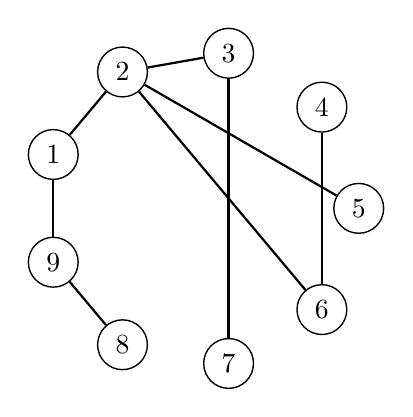
\begin{tikzpicture}
        \GraphInit[vstyle=Normal]
        \SetGraphUnit{2}
        \Vertices{circle}{5,4,3,2,1,9,8,7,6}
        \Edges(8,9,1,2,5)
        \Edges(2,3,7)
        \Edges(4,6)
        \Edges(2,6)
    \end{tikzpicture}
\end{minipage}
\end{center}


\end{questions}
\end{document}
